\documentclass{subfiles}
\begin{document}
    We will now guide you through the building process of the bank. The information provided here is not to scale and should only be used as a reference. Whilst building we will refer to the pieces as defined in the list of materials. When cutting the wood, we will introduce subpieces, which we define accordingly for better referencing. We strongly advice to write the names onto the pieces to avoid confusion while building. We will start by \emph{cutting}.

    \subsection{Cutting}
        This section contains schematics advising you on how to cut the wood. Do not follow these instructions without experience. We strongly advice to ask a professional for help. We do not take any responsibility for any damage or injury caused during the entire building process.

    \subsubsection*{Main board}
    Firstly we start with the founding piece of the bank. Cut two 20x18\SI{}{\square\centi\meter} pieces from W1.
    We will later use the rest of the wood to cut additional pieces. For reference we will call the two pieces W1.1 and W1.2.
    \begin{figure}[H]
        \centering
        \begin{tikzpicture}
            \coordinate (A) at (-6.725,-1.9);
            \coordinate (B) at (6.725,-1.9);
            \coordinate (C) at (6.725,1.9);
            \coordinate (D) at (-6.725,1.9);

            \coordinate (C1) at (-6.725,0.1);
            \coordinate (C2) at (-4.725,0.1);
            \coordinate (C3) at (-4.725,1.9);

            \coordinate (D1) at (6.725,0.1);
            \coordinate (D2) at (4.725,0.1);
            \coordinate (D3) at (4.725,1.9);

            \draw[] (A) -- (B) -- (C) -- (D) -- cycle;
            \draw[] (C1) -- (C2) -- (C3);
            \draw[] (D1) -- (D2) -- (D3);

            \coordinate (Am) at ($(A) + (0,-0.3)$);
            \coordinate (Bm) at ($(B) + (0,-0.3)$);
            \coordinate (Cm) at ($(C) + (0,0.3)$);
            \coordinate (Dm) at ($(D) + (0,0.3)$);

            \coordinate (mA) at ($(A) + (-0.3,0)$);
            \coordinate (mB) at ($(B) + (0.3,0)$);
            \coordinate (mC) at ($(C) + (0.3,0)$);
            \coordinate (mD) at ($(D) + (-0.3,0)$);

            \coordinate (C1m) at ($(C1) + (0,-0.3)$);
            \coordinate (C2m) at ($(C2) + (0,-0.3)$);
            \coordinate (C22m) at ($(C2) + (0.3,0)$);
            \coordinate (C3m) at ($(C3) + (0.3,0)$);

            \coordinate (D1m) at ($(D1) + (0,-0.3)$);
            \coordinate (D2m) at ($(D2) + (0,-0.3)$);
            \coordinate (D22m) at ($(D2) + (-0.3,0)$);
            \coordinate (D3m) at ($(D3) + (-0.3,0)$);

            \draw[<->] (Am) -- (Bm) node[pos=0.5,below] {$134.5\si{\cm}$};
            \draw[<->] (Cm) -- (Dm) node[pos=0.5,above] {$134.5\si{\cm}$};

            \draw[<->] (mA) -- (mD) node[pos=0.5,left] {$38\si{\cm}$};
            \draw[<->] (mB) -- (mC) node[pos=0.5,right] {$38\si{\cm}$};

            \draw[<->] (C1m) -- (C2m) node[pos=0.5,below] {$20\si{\cm}$};
            \draw[<->] (C22m) -- (C3m) node[pos=0.5,right] {$18\si{\cm}$};
            \draw[<->] (D22m) -- (D3m) node[pos=0.5,left] {$18\si{\cm}$};
            \draw[<->] (D1m) -- (D2m) node[pos=0.5,below] {$20\si{\cm}$};
        \end{tikzpicture}
        \caption{Scale is 1:10.}
    \end{figure}


    \subsection*{Triangle - Wall Protections}
    We will now cut two long 20x4\SI{}{\square\centi\meter} wood on both side of W1.1. The goal is to 
    provide a protection between the wall and the metal triangles. For reference we will call the two pieces W1.1.1 and W1.1.2.
    \begin{figure}[h]
        \centering
        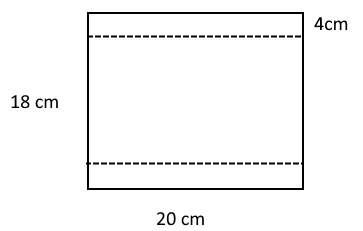
\includegraphics[width=0.5\textwidth]{Ressources/Cut_W1_1.png}
        \label{fig:Cut_W1_1}
        \caption{Cut two long 20x4\SI{}{\square\centi\meter} wood on both side of W1.1}
    \end{figure}

    \subsection*{Rear Support}
    We need support for the bank whene you on the rear of it to avoid falling back. 
    These piecies are fixed under the board and take support on the fixations of the railling to the walls. 
    We will now cut two small 10x5\SI{}{\square\centi\meter} wood in the rest of W1.1.
    \begin{figure}[h]
        \centering
        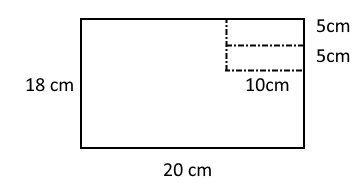
\includegraphics[width=0.5\textwidth]{Ressources/Cut_W1_2.png}
        \label{fig:Cut_W1_2}
        \caption{Cut two long 10x5\SI{}{\square\centi\meter} wood on both side of W1.2}
    \end{figure}
    You get two pieces that we define as W1.2.1 and W1.2.2.
\end{document}